\chapter{Neural Network ဆိုတာဘာလဲ?}

Neural network ဆိုတာ data ကိုသင်ယူပြီး အဖြေတွေထုတ်ပေးတဲ့ function ဖြစ်တယ်။
အခု လက်ရှိခေတ်မှာ AI လို့ပြောလိုက်ရင် Language model တွေကိုပဲ အများစု ရည်ညွှန်းတာ ဖြစ်နေပြီ။
Language model တွေဟာ neural network အမျိုးအစားတစ်ခုပဲ ဖြစ်တယ်။
တကယ်တော့ AI တွေဆိုတာ neural network တစ်မျိုးထဲတော့ မဟုတ်ဘူး။

ဒီစာအုပ်မှာတော့ AI လို့ပြောလိုက်ရင် neural network လို့ပဲ သတ်မှတ်ကြပါစို့။

\section{Decision Boundary}

အခုဆို dataset တစ်ခုပေးထားတယ်။ သူ့မှာ feature နှစ်ခုပါတယ်။ $x_1$, $x_2$ ဆိုပြီး။ output class က \redcircle\ ဒါမှမဟုတ် \bluecross\ ဖြစ်မယ်။
ဒါကတော့ ဥပမာ အနေနဲ့ ဖန်တီးပေးထားတာ။ တကယ့် data အစစ်တွေမဟုတ်ဘူး။
\begin{table}[H]
\centering
\begin{tabular}{ccc}
\hline
$x_1$ & $x_2$ & Class \\
\hline
1.0 & 1.0 & \tikz\draw[red, line width=1.5pt] (0,0) circle (4pt); \\
1.5 & 2.0 & \tikz\draw[red, line width=1.5pt] (0,0) circle (4pt); \\
2.0 & 1.5 & \tikz\draw[red, line width=1.5pt] (0,0) circle (4pt); \\
4.0 & 3.0 & \tikz\draw[blue, line width=2pt] (-4pt,-4pt) -- (4pt,4pt) (4pt,-4pt) -- (-4pt,4pt); \\
4.5 & 4.0 & \tikz\draw[blue, line width=2pt] (-4pt,-4pt) -- (4pt,4pt) (4pt,-4pt) -- (-4pt,4pt); \\
3.5 & 3.5 & \tikz\draw[blue, line width=2pt] (-4pt,-4pt) -- (4pt,4pt) (4pt,-4pt) -- (-4pt,4pt); \\
\hline
\end{tabular}
\caption{Training Dataset}
\end{table}

\noindent အခု dataset ကို အောက်ကအတိုင်း graph ဆွဲကြည့်လိုရတယ်။ အဲတာမျိုး data တွေကို နားလည်လွယ်အောင်၊ မြင်အောင်ကြည့်တာကို
data visualization လို့ခေါ်ပါတယ်။

\begin{figure}[h]
\centering
    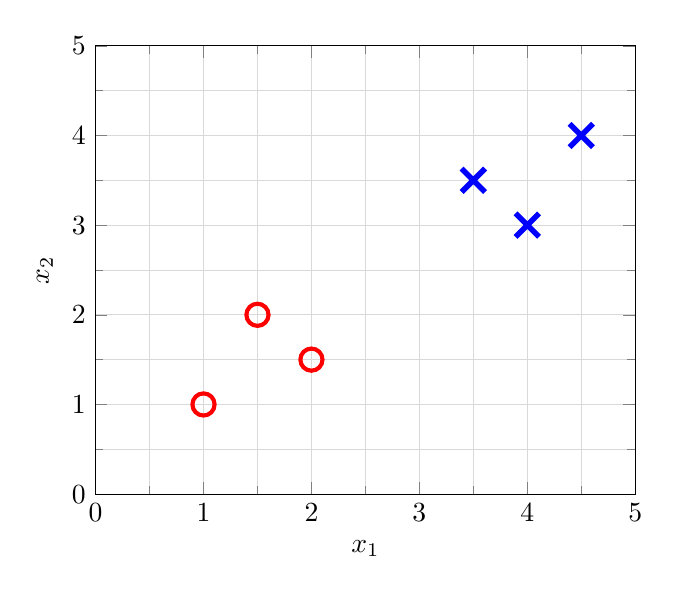
\begin{tikzpicture}
        \begin{axis}[
        xlabel={$x_1$}, ylabel={$x_2$},
        xmin=0, xmax=5, ymin=0, ymax=5,
        grid=both,
        grid style={line width=0.3pt, draw=gray!30},
        minor tick num=1,
        ]
        % Big Circle - Class 0
        \addplot[only marks, mark=o, mark size=4pt,
                line width=1.5pt, red]
        coordinates {(1,1)(1.5,2)(2,1.5)};

        % Big X - Class 1
        \addplot[only marks, mark=x, mark size=6pt,
                line width=2pt, blue]
        coordinates {(4,3)(4.5,4)(3.5,3.5)};
        \end{axis}
    \end{tikzpicture}
\caption{train dataset visualization}
\end{figure}

\noindent ကျွန်တော်တို့ model က ဒီ data တွေအားလုံးကို မှန်အောင်သင်ယူရမှာ ဖြစ်ပါတယ်။
ဒီလိုမျိုး အမျိုးအစားတွေ ခွဲခြားပေးတဲ့ neural network model ကို classification model လို့ခေါ်တယ်။
classification model တွေက ဘာလုပ်ပေးသလဲဆိုတော့ မတူတဲ့ အမျိုးအစား (class) တွေကြားမှာ နယ်နိမိတ်ဆွဲပေးတာဖြစ်တယ်။
\redcircle\ နဲ့ \bluecross ကို ခွဲခြားပေးဖို့ မျဥ်းဆွဲကြည့်ရအောင်။ အောက်မှာဖြစ်နိုင်တဲ့ model တွေပေးထားတယ်။

\begin{figure}[h]
\centering

\begin{subfigure}[b]{0.45\textwidth}
\centering
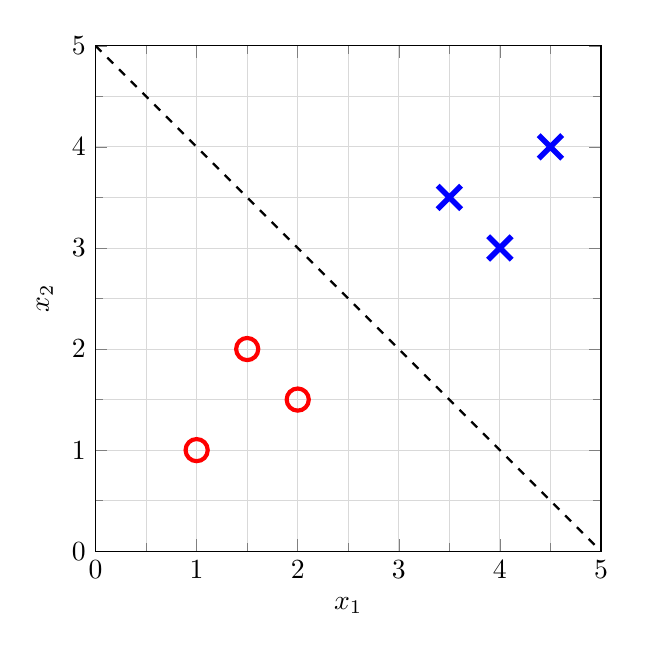
\begin{tikzpicture}
\begin{axis}[
  xlabel={$x_1$}, ylabel={$x_2$},
  xmin=0, xmax=5, ymin=0, ymax=5,
  grid=both,
  grid style={line width=0.3pt, draw=gray!30},
  minor tick num=1,
  width=8cm, height=8cm,
]
\addplot[only marks, mark=o, mark size=4pt,
         line width=1.5pt, red]
  coordinates {(1,1)(1.5,2)(2,1.5)};
\addplot[only marks, mark=x, mark size=6pt,
         line width=2pt, blue]
  coordinates {(4,3)(4.5,4)(3.5,3.5)};
% Decision boundary: x2 = x1
\addplot[domain=0:5, samples=2, thick, black, dashed]
  {-x + 5};
\end{axis}
\end{tikzpicture}
\end{subfigure}
\hfill
\begin{subfigure}[b]{0.45\textwidth}
\centering
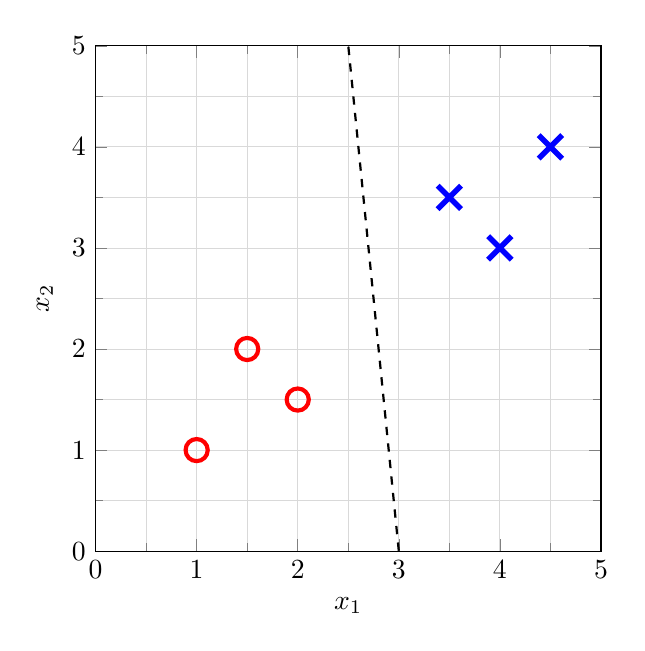
\begin{tikzpicture}
\begin{axis}[
  xlabel={$x_1$}, ylabel={$x_2$},
  xmin=0, xmax=5, ymin=0, ymax=5,
  grid=both,
  grid style={line width=0.3pt, draw=gray!30},
  minor tick num=1,
  width=8cm, height=8cm,
]
\addplot[only marks, mark=o, mark size=4pt,
         line width=1.5pt, red]
  coordinates {(1,1)(1.5,2)(2,1.5)};
\addplot[only marks, mark=x, mark size=6pt,
         line width=2pt, blue]
  coordinates {(4,3)(4.5,4)(3.5,3.5)};
% Decision boundary: x2 = -x1 + 5
\addplot[domain=0:5, samples=2, thick, black, dashed]
  {-10 * x + 30};
\end{axis}
\end{tikzpicture}
\end{subfigure}

\vspace{1em}

\begin{subfigure}[b]{0.45\textwidth}
\centering
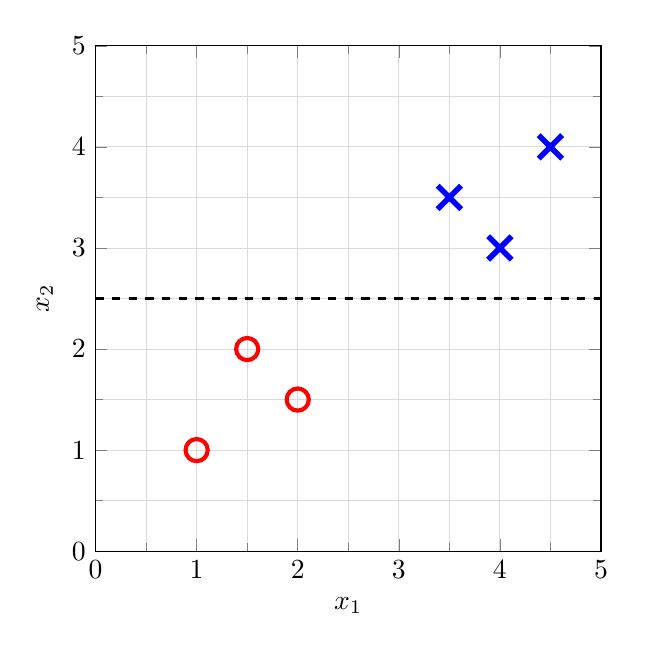
\begin{tikzpicture}
\begin{axis}[
  xlabel={$x_1$}, ylabel={$x_2$},
  xmin=0, xmax=5, ymin=0, ymax=5,
  grid=both,
  grid style={line width=0.3pt, draw=gray!30},
  minor tick num=1,
  width=8cm, height=8cm,
]
\addplot[only marks, mark=o, mark size=4pt,
         line width=1.5pt, red]
  coordinates {(1,1)(1.5,2)(2,1.5)};
\addplot[only marks, mark=x, mark size=6pt,
         line width=2pt, blue]
  coordinates {(4,3)(4.5,4)(3.5,3.5)};
\addplot[domain=0:5, samples=2, thick, black, dashed]
  {2.5};
\end{axis}
\end{tikzpicture}
\end{subfigure}
\hfill
\begin{subfigure}[b]{0.45\textwidth}
\centering
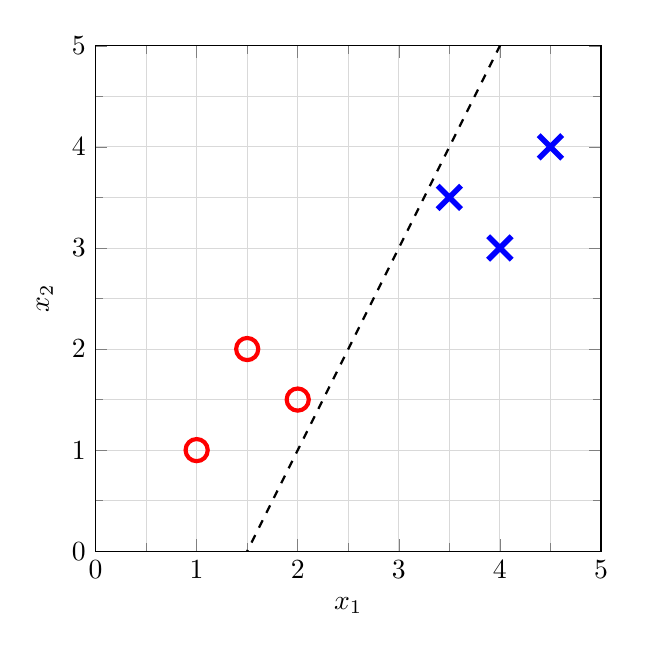
\begin{tikzpicture}
\begin{axis}[
  xlabel={$x_1$}, ylabel={$x_2$},
  xmin=0, xmax=5, ymin=0, ymax=5,
  grid=both,
  grid style={line width=0.3pt, draw=gray!30},
  minor tick num=1,
  width=8cm, height=8cm,
]
\addplot[only marks, mark=o, mark size=4pt,
         line width=1.5pt, red]
  coordinates {(1,1)(1.5,2)(2,1.5)};
\addplot[only marks, mark=x, mark size=6pt,
         line width=2pt, blue]
  coordinates {(4,3)(4.5,4)(3.5,3.5)};
% Decision boundary: x2 = -x1 + 5
\addplot[domain=0:5, samples=2, thick, black, dashed]
  {2 * x - 3};
\end{axis}
\end{tikzpicture}
\end{subfigure}

\caption{မှန်ကန်သော model များ}
\end{figure}
\clearpage

အပေါ်က model ၄ခုလုံးက ပေးထားတဲ့ train dataset တစ်ခုလုံးကို မှန်အောင်လုပ်ပေးနိုင်တဲ့ model တွေ ဖြစ်ကြတယ်။
အဲဒီလို data class တွေကို ပိုင်းခြားပေးတဲ့ မျဥ်းကို decision boundary လို့ခေါ်တယ်။ အဲတာဆို အဲဒီထဲမှာ ဘယ် model က အကောင်းဆုံးလဲ?

မြင်သာအောင် ပြောရင် သိသိသာသာ အလယ်ရောက်လေလေ ကောင်းလေပေါ့။ \redcircle\ နဲ့ \bluecross\ တစ်ခုစီသာရှိခဲ့မယ်ဆိုရင် သူတို့နှစ်ခုရင် အလယ် ဗဟိုမှာ မျဥ်းဆွဲလိုက်ရင် ဘက်မလိုက် (unbiased) တော့ဘူးပေါ့။ ဒါကတော့ မြင်သာအောင် အလွယ်ပြောလိုက်တာ။ ဘယ်ဟာမှ မရွေးခင် စမ်းသပ်မဲ့ test dataset ကို ကြည့်ကြရအောင်။

\begin{table}[H]
\centering
\begin{tabular}{ccc}
\hline
$x_1$ & $x_2$ & Class \\
\hline
2.5 & 4.0 & \tikz\draw[red, line width=1.5pt] (0,0) circle (4pt); \\
3.0 & 0.5 & \tikz\draw[blue, line width=2pt] (-4pt,-4pt) -- (4pt,4pt) (4pt,-4pt) -- (-4pt,4pt); \\
\hline
\end{tabular}
\caption{Test Dataset}
\end{table}

အောက်မှာ test dataset ကို model ၄ခုနဲ့ စမ်းထားတဲ့ပုံတွေ ပြထားပါတယ်။
အခုလို test dataset နဲ့ စမ်းကြည့်လိုက်တဲ့အခါ် model တိုင်းက မမှန်တော့ဘူး။ ဒီမှာတော့ တစ်ချို့ model တွေကို
သေချာမှားအောင် ရွေးပြီး test data ကို ထည့်ပေးထားတာ။ ဒီလိုလုပ်ရတဲ့ ရည်ရွယ်ချက်က AI model တွေကို
သင်ပေးရတဲ့ နေရာမှာ ဖြစ်တတ်တဲ့ သဘောတရားတွေကို မြင်စေချင်လို့။

neural network တွေဟာ ပင်ကိုယ်အားဖြင့် အသိဉာဏ်လုံးဝ မရှိဘူး။ သူတို့ရဲ့တစ်ခုထဲသော အလုပ်က
သင်ရမဲ့ train dataset ကို မှန်အောင် သင်ယူဖို့ပဲ ဖြစ်တယ်။ အခုဆို သဘောတရားအားဖြင့် ပေးထားတဲ့ model 
၄ခုလုံးက သင်ယူတဲ့နေရာမှာ တာဝန်ကျေကြတယ်။ ဒီဆိုဘာလို့ အားလုံး test dataset ပေါ်မှာ မအောင်မြင်ကြလဲ?

ဒီစာအုပ်မှာတော့ ဖတ်တဲ့သူတွေကို ပညာရပ်သာမကပဲ အတွေးအခေါ်ပါရစေချင်တယ်။ ဒီကြောင့် စဥ်းစားကြည့်ပါ။
neural network တွေအသုံးမကျရင် သူတို့ကိုချည်းပဲ အပြစ်တင်သင့်လား?

တကယ့်လက်တွေမှာတော့ model တွေကို ပိုကောင်းစေချင်ရင် data အများကြီးသုံးကြတယ်။
data အများကြီးကို နယ်နိမိတ်တွေ ဆွဲပေးရင် စမ်းသပ်တဲ့အခါမှာလဲ test dataset ထဲက example တွေက
အဲဒီ သင်ထားတဲ့ နယ်ခြားတွေထဲမှာ ရောက်ဖို့ ပိုသေချာတယ်။ အဲတာဆို test dataset တွေကိုလဲ
မှန်အောင် အဖြေထုတ်ပေးနိုင်တယ်ပေါ့။

ဒါကတော့ model training နဲ့ သူတို့ရဲ့ သဘောသဘာဝ အခြေခံပါပဲ။ အခုလောလောဆယ်တော့ ဒီလောက်ပဲ မှတ်ထားပါ။

\begin{figure}[H]
\centering

\begin{subfigure}[b]{0.45\textwidth}
\centering
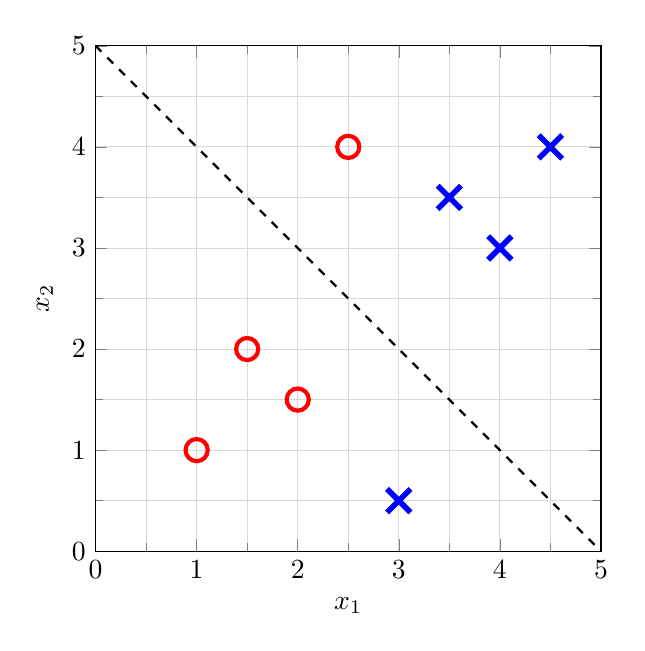
\begin{tikzpicture}
\begin{axis}[
  xlabel={$x_1$}, ylabel={$x_2$},
  xmin=0, xmax=5, ymin=0, ymax=5,
  grid=both,
  grid style={line width=0.3pt, draw=gray!30},
  minor tick num=1,
  width=8cm, height=8cm,
]
\addplot[only marks, mark=o, mark size=4pt,
         line width=1.5pt, red]
  coordinates {(1,1)(1.5,2)(2,1.5)(2.5,4.0)};
\addplot[only marks, mark=x, mark size=6pt,
         line width=2pt, blue]
  coordinates {(4,3)(4.5,4)(3.5,3.5)(3.0,0.5)};
% Decision boundary: x2 = x1
\addplot[domain=0:5, samples=2, thick, black, dashed]
  {-x + 5};
\end{axis}
\end{tikzpicture}
\end{subfigure}
\hfill
\begin{subfigure}[b]{0.45\textwidth}
\centering
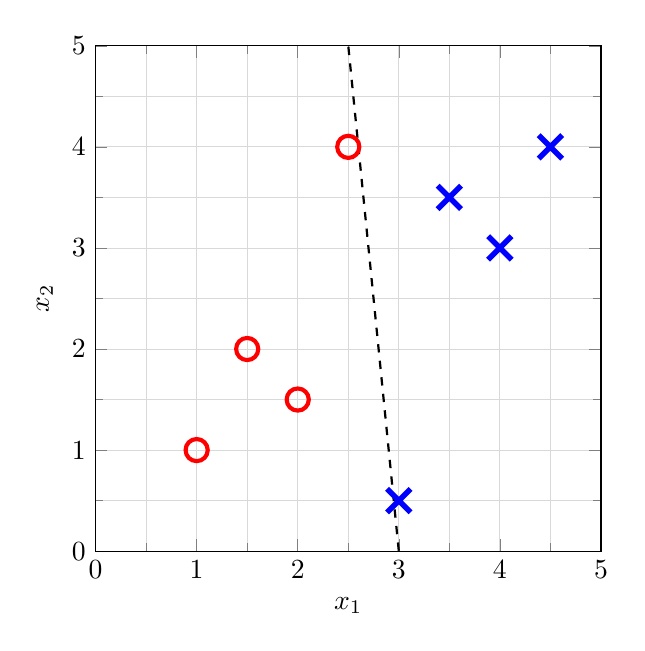
\begin{tikzpicture}
\begin{axis}[
  xlabel={$x_1$}, ylabel={$x_2$},
  xmin=0, xmax=5, ymin=0, ymax=5,
  grid=both,
  grid style={line width=0.3pt, draw=gray!30},
  minor tick num=1,
  width=8cm, height=8cm,
]
\addplot[only marks, mark=o, mark size=4pt,
         line width=1.5pt, red]
  coordinates {(1,1)(1.5,2)(2,1.5)(2.5,4.0)};
\addplot[only marks, mark=x, mark size=6pt,
         line width=2pt, blue]
  coordinates {(4,3)(4.5,4)(3.5,3.5)(3.0,0.5)};
% Decision boundary: x2 = -x1 + 5
\addplot[domain=0:5, samples=2, thick, black, dashed]
  {-10 * x + 30};
\end{axis}
\end{tikzpicture}
\end{subfigure}

\vspace{1em}

\begin{subfigure}[b]{0.45\textwidth}
\centering
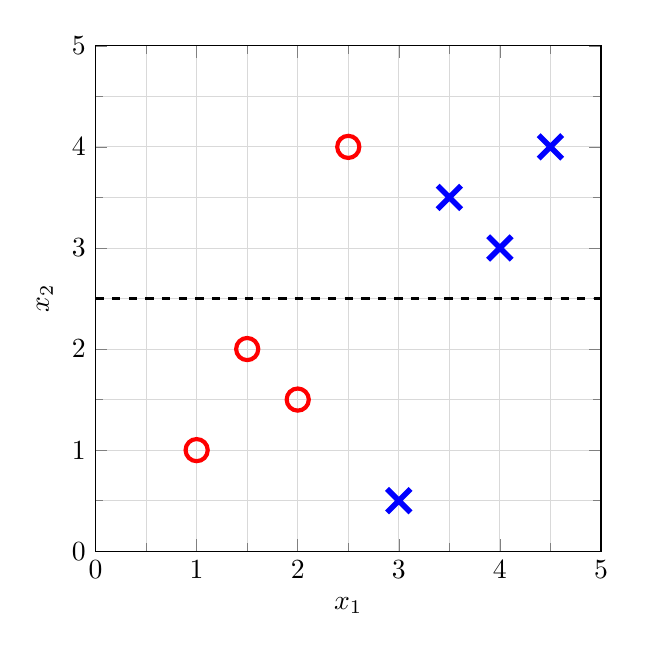
\begin{tikzpicture}
\begin{axis}[
  xlabel={$x_1$}, ylabel={$x_2$},
  xmin=0, xmax=5, ymin=0, ymax=5,
  grid=both,
  grid style={line width=0.3pt, draw=gray!30},
  minor tick num=1,
  width=8cm, height=8cm,
]
\addplot[only marks, mark=o, mark size=4pt,
         line width=1.5pt, red]
  coordinates {(1,1)(1.5,2)(2,1.5)(2.5,4.0)};
\addplot[only marks, mark=x, mark size=6pt,
         line width=2pt, blue]
  coordinates {(4,3)(4.5,4)(3.5,3.5)(3.0,0.5)};
\addplot[domain=0:5, samples=2, thick, black, dashed]
  {2.5};
\end{axis}
\end{tikzpicture}
\end{subfigure}
\hfill
\begin{subfigure}[b]{0.45\textwidth}
\centering
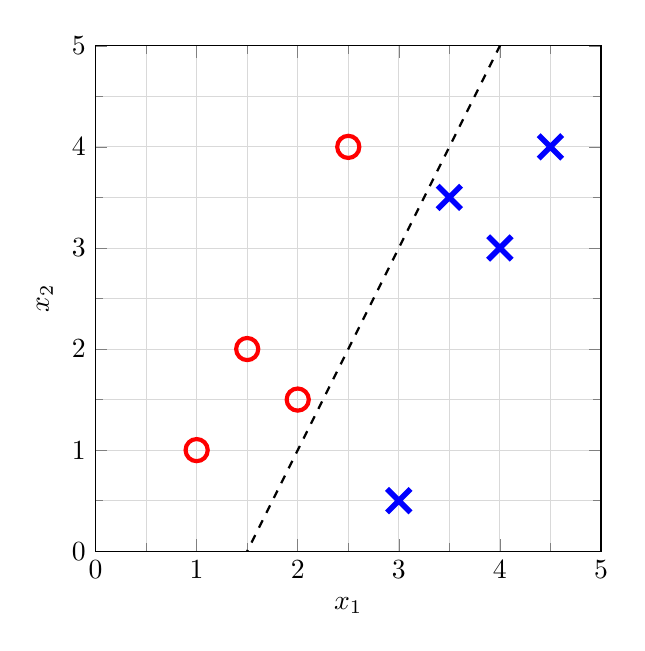
\begin{tikzpicture}
\begin{axis}[
  xlabel={$x_1$}, ylabel={$x_2$},
  xmin=0, xmax=5, ymin=0, ymax=5,
  grid=both,
  grid style={line width=0.3pt, draw=gray!30},
  minor tick num=1,
  width=8cm, height=8cm,
]
\addplot[only marks, mark=o, mark size=4pt,
         line width=1.5pt, red]
  coordinates {(1,1)(1.5,2)(2,1.5)(2.5,4.0)};
\addplot[only marks, mark=x, mark size=6pt,
         line width=2pt, blue]
  coordinates {(4,3)(4.5,4)(3.5,3.5)(3.0,0.5)};
% Decision boundary: x2 = -x1 + 5
\addplot[domain=0:5, samples=2, thick, black, dashed]
  {2 * x - 3};
\end{axis}
\end{tikzpicture}
\end{subfigure}

\caption{model တစ်ခုချင်းစီကို train dataset + test dataset နဲ့ စမ်းထားပုံ}
\end{figure}
